%% ------------------------------------------------------------------------- %%
\chapter{Questionário às comunidades}
\label{cap:pesquisas}

% TODO tentar mostrar mais uma relação no sentido FLOSS -> M.A.
% No mínimo, ter os argumentos para responder a eventuais perguntas
% que sugiram isso

O trabalho apresentado até agora dá indícios de que há uma ligação
implícita forte entre as comunidades de software livre e de métodos
ágeis. No entanto fica claro que ainda existem várias possibilidades
para melhorias nessa relação. Num primeiro passo, para delinear a
situação atual das comunidades e identificar problemas e soluções
desejados por cada lado, foram elaborados dois questionários.

O objetivo desses questionários era obter informações das comunidades
envolvidas com relação a comportamentos e ferramentas comuns no
processo de desenvolvimento. No contexto de métodos ágeis, era
importante entender a proporção de pessoas com experiências em
projetos ágeis distribuídos e como essa distribuição afetou o
desenvolvimento tanto no aspecto ferramental quanto
comportamental. Esse interesse pela distribuição das equipes se deve
ao fato de que projetos livres costumam enfrentar esse tipo de
ambiente. Os dados coletados serviriam para delinear as práticas
comuns das comunidades e os pontos de diferenças a serem estudados.

A Seção~\ref{sec:questionarios} apresenta os questionários elaborados
para a comunidade de software livre e a comunidade de métodos
ágeis. Em seguida, a Seção~\ref{sec:respostas} apresenta uma análise
dos dados obtidos pelas respostas. Finalmente, a
Seção~\ref{sec:proposta} apresenta uma conclusão da análise dos dados.

\section{Os questionários}
\label{sec:questionarios}

Cada questionário foi elaborado de forma a caracterizar o público
participante e foi direcionado a apenas uma comunidade. Ambos
questionários foram elaborados como formulários em uma página na
Internet e foram divulgados em canais correspondentes a cada uma das
comunidades. A Seção~\ref{subsec:floss} apresenta o questionário
elaborado para contribuidores de software livre enquanto a
Seção~\ref{subsec:agile} apresenta a versão apresentada à comunidade
de métodos ágeis.

\subsection{Para a comunidade de software livre}
\label{subsec:floss}

Em ambos questionários, houve um trabalho para tentar caracterizar a
população que respondeu ao questionário e quão representativa essa
população era de sua comunidade. Portanto, o primeiro conjunto de
perguntas era bem semelhante nas duas pesquisas. Os questionários
também trouxeram perguntas que tentavam avaliar a experiência dos
participantes em suas comunidades. No caso da comunidade de software
livre, essas perguntas abordaram a quantidade de projetos com os quais
o participante contribuiu e quando sua primeira contribuição
aconteceu.

Essa última pergunta e as seguintes eram exibidas apenas aos
participantes que declararam ter contribuído com, pelo menos, um
projeto de software livre. Esse comportamento visou minimizar o
trabalho dos participantes assim como reduzir a quantidade de
respostas sem sentido no questionário. De forma a minimizar o ambiente
que os participantes deveriam avaliar assim como descobrir sua
experiência no projeto avaliado, o questionário perguntava o nome do
principal projeto de software livre com o qual o participante
contribui (ou contribuía) e o papel do participante nesse projeto.

Para entender como o projeto assegurava a comunicação entre seus
colaboradores, os participantes deviam responder quão grande era a
equipe do projeto e, no caso da equipe ter mais do que um integrante,
qual canal de comunicação era usado entre os membros da equipe. O
questionário também pedia ao participante que avaliasse a qualidade da
comunicação através desse canal e no canal usado para comunicação com
os usuários.  Por fim, o questionário perguntava que ferramentas,
dentre oito sugeridas, o projeto já tinha usado e como eles avaliam a
utilidade dessas ferramentas para abrandar seus problemas com o
desenvolvimento do projeto.

% TODO Agrupar e resumir os tipos de portais.

O Apêndice~\ref{ape:OS} apresenta uma versão traduzida para o
Português e adaptada para papel do questionário que foi
disponibilizado na
Internet\footnote{\url{http://www.ime.usp.br/~corbucci/floss-survey}
  -- Último acesso em 24/01/2011}. As chamadas à participação no
questionário foram divulgadas em diversos canais ligados à comunidade
de software livre. Um canal forte de divulgação foi o
Twitter\footnote{\url{http://twitter.com} -- Último acesso em
  24/01/2011} graças à ajuda do portal
GitHub\footnote{\url{http://www.github.com} -- Último acesso em
  24/01/2011} que enviou uma mensagem divulgando o questionário a
todos seus seguidores. O questionário também foi enviado a outros
portais incubadores de projetos livres como
SourceForge.net\footnote{\url{http://www.sourceforge.net} -- Último
  acesso em 24/01/2011},
LaunchPad.net\footnote{\url{http://launchpad.net} -- Último acesso em
  24/01/2011}, CodeHaus\footnote{\url{http://codehaus.org} -- Último
  acesso em 24/01/2011} e Google
Code\footnote{\url{http://code.google.com} -- Último acesso em
  24/01/2011} mas nenhum respondeu aos pedidos. Além disso, alguns
blogs e listas de emails de comunidades livres tiveram divulgações por
parte de seus membros sobre o questionário tanto no âmbito nacional
quanto internacional.

A próxima seção apresenta as diferenças entre este questionário e o
questionário divulgado na comunidade de métodos ágeis.

\subsection{Para praticantes de métodos ágeis}
\label{subsec:agile}

Conforme descrito na Seção~\ref{subsec:floss}, o começo do
questionário direcionado à comunidade de métodos ágeis era muito
semelhante ao outro, já que visava obter informações genéricas para
traçar o perfil dos participantes.  Após essas primeiras perguntas
sobre o país de residência e o ano de nascimento, o questionário
perguntava aos participantes em quantos projetos ágeis eles já haviam
participado e quando foi sua primeira experiência em um projeto ágil.
De forma semelhante ao questionário para a comunidade de software
livre, essa última pergunta, assim como as seguintes, era apresentada
apenas aos participantes que disseram ter participado em pelo menos um
projeto ágil.

Em seguida, o participante devia informar seu papel no principal
projeto ágil que participou e o tamanho da equipe envolvida. O
questionário continuava perguntando qual era o principal canal de
comunicação usado para falar com o cliente do projeto assim como a
qualidade desse canal.

Diferentemente da pesquisa para projetos livres, a próxima pergunta
questionava se o participante já tinha tido alguma experiência com
métodos ágeis em um ambiente distribuído. Caso a resposta fosse
afirmativa, o questionário apresentava duas perguntas para identificar
o principal canal de comunicação entre a equipe e a qualidade
percebida desse canal.

Feito isso, os participantes deviam ordenar uma lista de oito
problemas para apontar os três mais críticos que eles encontraram nos
ambientes ágeis em que participaram. De forma semelhante, os
participantes ordenavam, em seguida, oito ferramentas que eles
acreditavam que poderiam ajudar em ambientes de desenvolvimento
distribuído de forma a selecionar as três mais importantes.

Por fim, os participantes tinham que informar se eram contribuidores
de projetos de software livre e, se fossem, quão ágil eles
consideravam seus projetos livres. Apenas caso fossem contribuidores,
as perguntas relacionadas aos problemas e às ferramentas eram
repetidas pedindo para o participante considerar o contexto do
principal projeto livre com o qual contribuiu (ou contribuía).

O Apêndice~\ref{ape:MA} apresenta uma versão em papel e em Português
do questionário digital que foi disponibilizado na
Internet\footnote{\url{http://www.ime.usp.br/~corbucci/agile-survey}
  -- Último acesso em 24/01/2011}|. Esse questionário foi divulgado
(num período diferente do outro, conforme apresentado na Seção
\ref{sec:respostas}) por e-mail em listas de discussões sobre métodos
ágeis nacionais e internacionais e através do sistema Twitter por
diversas pessoas. Os autores também buscaram apoio da Agile
Alliance\footnote{\url{http://www.agilealliance.org} -- Último acesso
  em 28/10/2010} mas não houve nenhuma resposta em nome da entidade.

\section{Respostas aos questionários}
\label{sec:respostas}

% TODO Informacao do erro de JS no IE, relevante? Talvez nao.
% Se for usar, achar um numero global.

Conforme foi dito anteriormente, os questionários foram elaborados com
o objetivo de serem respondidos via Internet. Por isso, o questionário
contava com alguns comportamentos dinâmicos que modificavam o
questionário de acordo com as respostas fornecidas. Para implementar
esse comportamento, foram usadas algumas rotinas escritas na linguagem
Javascript. Infelizmente, seu funcionamento só foi validado em
navegadores modernos. Navegadores antigos (como Internet Explorer
versão 6 e 7) não foram testados e descobriu-se posteriormente que o
preenchimento do questionário nesses navegadores resultava em
respostas inválidas. Esse erro inesperado acabou provendo informações
extras sobre os navegadores e versões usadas em cada uma das
comunidades. As próximas subseções apresentam uma análise dos dados
coletados em cada um dos questionários.

\subsection{Resultados da comunidade de software livre}
\label{sec:resp-floss}

As respostas para o questionário direcionado à comunidade de software
livre foram coletadas entre o dia 28 de Julho de 2009 e dia
1$^\textrm{o}$ de Novembro de 2009. Foram 309 respostas das quais 3
eram entradas duplicadas (mesmo endereço IP e horários e datas muito
próximos) enquanto 4 outras eram inválidas (causadas por erros de
Javascript devidos ao uso de navegadores antigos). Esses dados nos
mostram que aproximadamente 1\% das pessoas ligadas às comunidades de
software livre usam navegadores incompatíveis com os padrões atuais.

Das 302 entradas válidas restantes, 122 eram respostas nas quais o
participante afirmava nunca ter contribuído com um projeto de software
livre mas se sentia como parte da comunidade. Essa atitude mostra que
apenas cerca de 60\% da comunidade de software livre de fato contribui
com projetos.

% XXX Figuras ficam em páginas ruins de ler o texto associado

\begin{figure}[hbt]
  \begin{minipage}[t]{0.5\linewidth}
    \centering
    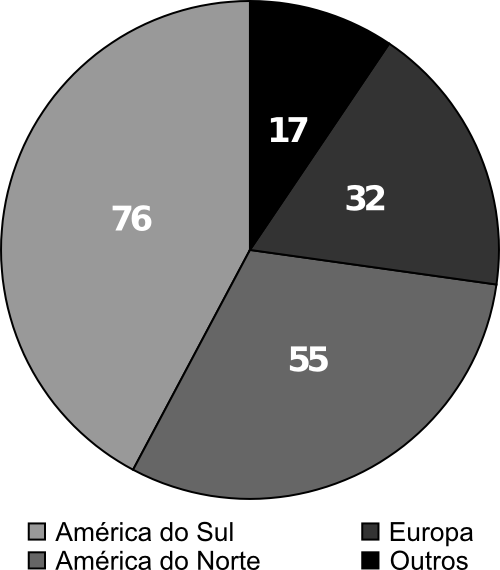
\includegraphics[scale=.8]{floss-world}
    \caption{Distribuição das respostas do questionário aos
      contribuidores de software livre por regiões}
    \label{fig:floss-world}
  \end{minipage}
  \begin{minipage}[t]{0.5\linewidth}
    \centering
    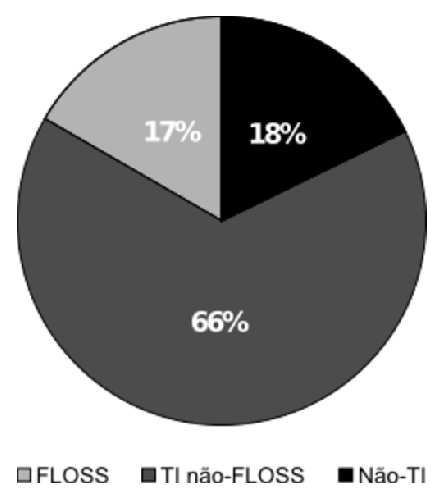
\includegraphics[scale=.8]{floss-income}
    \caption{Origem da renda principal dos contribuidores de software
      livre}
    \label{fig:floss-income}
  \end{minipage}
\end{figure}

O restante da análise foi realizado sobre as 180 respostas de
contribuidores efetivos já que elas apresentavam resultados mais
interessantes. A Figura~\ref{fig:floss-world} apresenta a distribuição
das respostas nas diferentes regiões do mundo. Vale notar que a
distribuição representa mais os locais em que o questionário foi
divulgado do que, de fato, a distribuição de participações em projetos
livres. A Figura~\ref{fig:floss-income} exibe as principais
classificações para origem da renda principal dos participantes do
questionário. É interessante notar que esses dados não divergem muito
dos resultados coletados por outras pesquisas~\cite{FlossStats}.

A idade média dos participantes do questionário é de 28 anos e a média
do primeiro ano de contribuição em projetos livres foi em 2003. A
Figura~\ref{fig:floss-firstxp} mostra que os contribuidores mais
jovens começaram a participar mais cedo em suas vidas do que os mais
velhos. Essa mudança pode ser explicada pela crescente facilidade de
acesso a computadores nos últimos anos.

% XXX Indicações do que representam os eixos

\begin{figure}
  \centering
  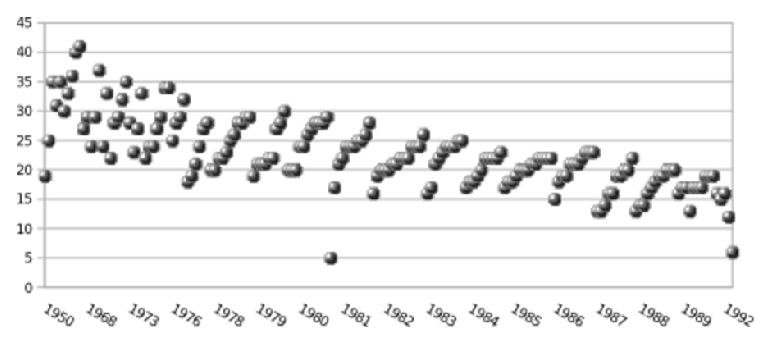
\includegraphics[scale=1]{floss-firstxp}
  \caption{Idade na época da primeira contribuição livre pelo ano de
    nascimento}
  \label{fig:floss-firstxp}
\end{figure}

Aproximadamente dois terços dos participantes se identificaram como
mantenedores de projetos, \textit{commiters} ou programadores. O
último terço se dividiu entre outros papéis como mostra a
Figura~\ref{fig:floss-roles}. Os tamanhos das equipes também foi bem
representativo já que apenas 6\% dos projetos eram desenvolvidos por
uma única pessoa enquanto 48\% reuniam até 6 pessoas. A
Figura~\ref{fig:floss-teams} mostra esses resultados e outros tamanhos
de equipes. É interessante notar que o perfil traçado pelas respostas
é similar ao perfil apresentado por Reis~\cite{Reis2003} obtido em
2003. Esse fato sugere que a amostra coletada é tão representativa da
comunidade de software livre quanto na pesquisa de Reis.

% XXX padronizar com valores absolutos e acertar "requisitor de
% funcionalidades"

% XXX Adicionar legenda no eixo Y da figura floss-teams

\begin{figure}[htb]
  \begin{minipage}[t]{0.55\linewidth}
    \centering
    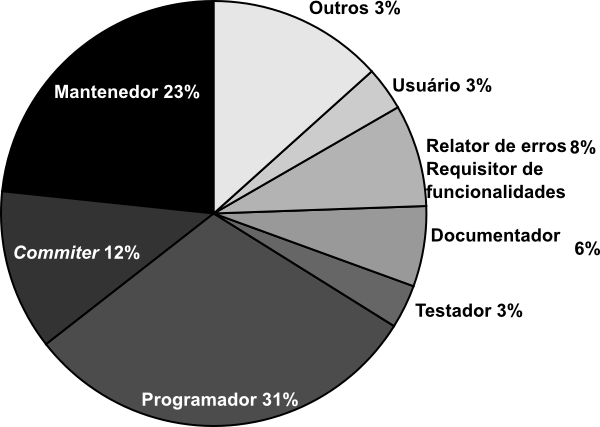
\includegraphics[scale=.9]{floss-roles}
    \caption{Distribuição dos papéis dos participantes nas equipes de
      projetos livres}
    \label{fig:floss-roles}
  \end{minipage}
  \begin{minipage}[t]{0.45\linewidth}
    \centering
    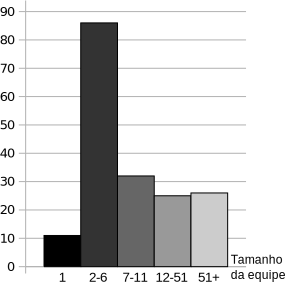
\includegraphics[scale=.75]{floss-teams}
    \caption{Tamanho das equipes apresentado pelos participantes}
    \label{fig:floss-teams}
  \end{minipage}
\end{figure}

Com relação aos principais canais de comunicação, parece que pouco
mudou desde as pesquisas de Reis ou do \textit{Floss world}. Os
principais canais de comunicação entre a equipe continuam sendo as
listas de correio eletrônico (27\%) e Papo Retransmitido pela Internet
(IRC - 23\%). No entanto a quantidade de pessoas usando comunicação
face a face entre as equipes aumentou (atualmente em 15\%).

A avaliação da qualidade de comunicação nesses canais foi
relativamente parecida. Listas de correio eletrônico foram avaliadas
como sendo 44\% eficazes contra 52\% para o papo retransmitido pela
Internet e 49\% para comunicação face a face. Parece que, com o
crescimento da adoção de canais de comunicação com curto tempo de
resposta via Internet, listas de correio eletrônico mostram sinais de
fraqueza se comparadas a outros canais com maior taxa de transferência
de informações.

Quando se trata de comunicação com os usuários, listas de correio
eletrônico foram as mais usadas (32\%) seguidas de páginas de Internet
(18\%) e canais IRC, correio eletrônico e sistemas de controle de
problemas (11\% cada). Quando se fala da qualidade desses canais de
comunicação, os canais IRC levam a melhor novamente com 49\% de
eficácia contra 44\% para listas de correio eletrônico, 37\% para
páginas na Internet, 33\% de ferramentas de rastreamento de problemas
e apenas 23\% para os correios eletrônicos.

Para ambos ambientes, outros canais de comunicação foram omitidos já
que a quantidade de respostas era muito pequena para ter alguma
relevância.

\begin{figure}
  \centering
  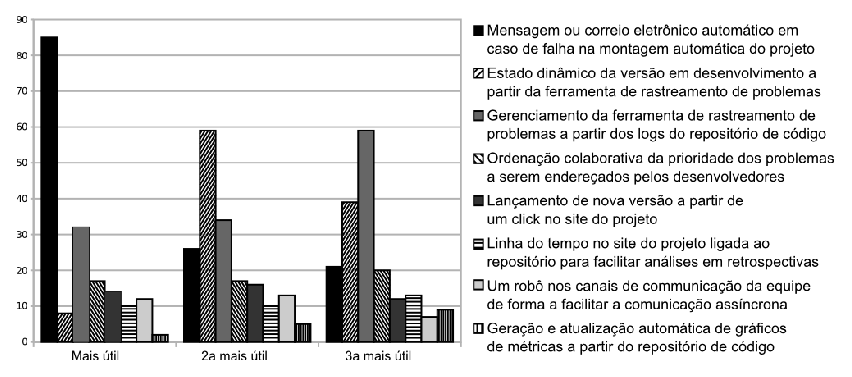
\includegraphics[scale=1.2]{floss-tools}
  \caption{Respostas sobre a utilidade de ferramentas para projetos de
    software livre}
  \label{fig:floss-tools}
\end{figure}

A Figura~\ref{fig:floss-tools} mostra as três ferramentas consideradas
as mais úteis em um projeto de software livre. Mensagem ou correio
eletrônico enviado automaticamente em caso de falha na construção do
software foi de longe considerada a ferramentas mais útil seguida por
um gráfico do estado do projeto gerado dinamicamente a partir da
ferramenta de rastreamento de problemas. Em terceiro lugar ficou uma
ferramenta que permite a gestão da ferramenta de rastreamento de
problemas a partir das mensagens de mudanças no repositório de código
do projeto.

\begin{figure}
  \centering
  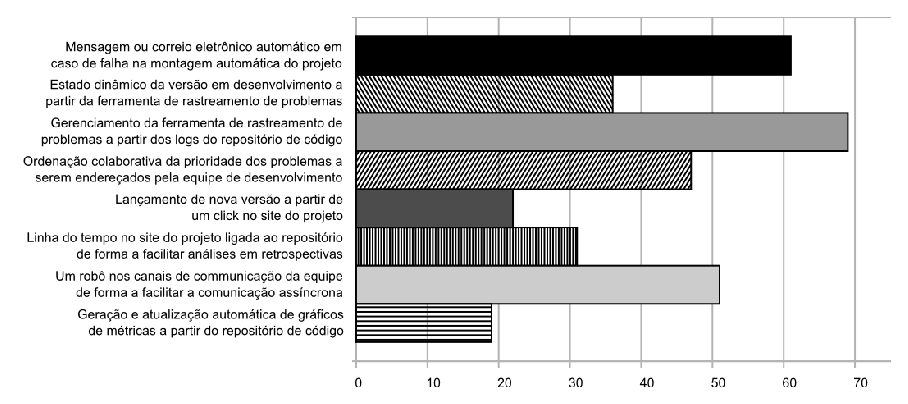
\includegraphics[scale=1]{floss-existingtools}
  \caption{Ferramentas que os participantes já usam em seus projetos
    livres}
  \label{fig:floss-existingtools}
\end{figure}

A Figura~\ref{fig:floss-existingtools} mostra que uma quantidade
razoável dos projetos já tem um sistema de mensagens ou correio
eletrônico em caso de falha na construção do projeto e um sistema de
gestão da ferramentas de controle de problemas através das mensagens
de mudança no repositório. No entanto, deve ser considerado que o
GitHub \footnote{\url{http://www.github.com} -- Último acesso em
  24/01/2011} oferece essa última ferramenta enquanto muitos outros
portais não oferecem. E dado que o GitHub divulgou oficialmente o
questionário, é provável que muitos de seus usuários responderam o
questionário. Portanto a amostra pode estar viciada nesse sentido.

\subsection{Resultados da comunidade de métodos ágeis}
\label{sec:resp-agile}

Os resultados para o questionário direcionado à comunidade de métodos
ágeis foram coletados entre 1$^{\textrm{o}}$ de Outubro de 2009 e
1$^{\textrm{o}}$ de Dezembro de 2009. Foram 204 respostas das quais 9
eram entradas duplicadas e 34 eram inválidas devido ao uso de
navegadores incompatíveis com o padrão da linguagem Javascript. Esses
dados mostram que aproximadamente 18\% da comunidade de métodos ágeis
ainda usa navegadores antigos e incompatíveis com os padrões
atuais. Esse valor é sensivelmente maior do que para a comunidade de
software livre.

Dessas 161 respostas válidas apenas 28 eram de pessoas que nunca
participaram de um projeto ágil mas se consideravam parte dos
praticantes de métodos ágeis. Essa medida é outra que difere bastante
dos resultados na comunidade de software livre. Ela pode indicar que a
comunidade de métodos ágeis valoriza muito mais experiência prática do
que a comunidade de software livre.

% XXX Legenda nos eixos da figura agile-xp

\begin{figure}[htb]
  \begin{minipage}[t]{0.45\linewidth}
    \centering
    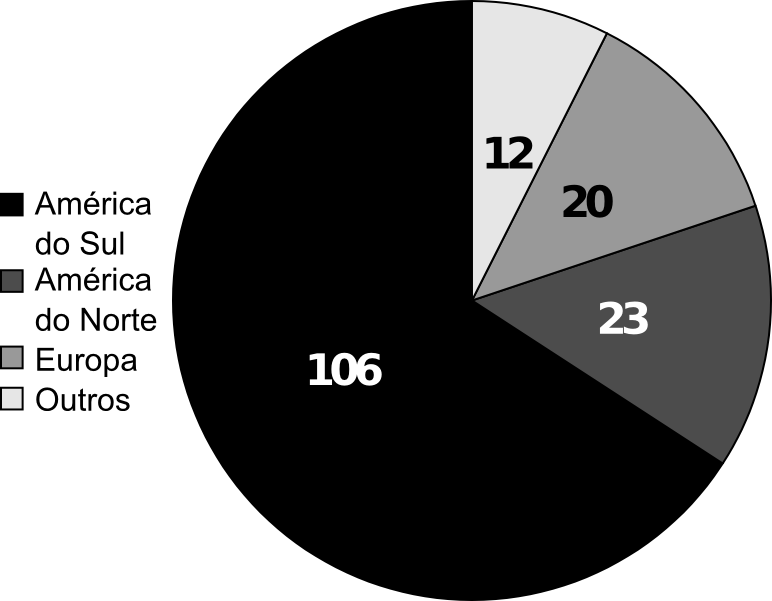
\includegraphics[scale=.65]{agile-world}
    \caption{Distribuição das respostas para praticantes de métodos
      ágeis agrupadas por regiões do mundo}
    \label{fig:agile-world}
  \end{minipage}
  \begin{minipage}[t]{0.55\linewidth}
    \centering
    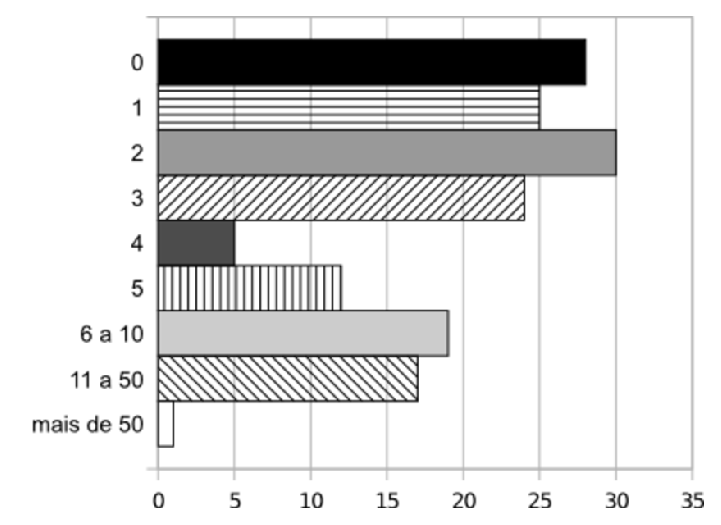
\includegraphics[scale=.7]{agile-xp}
    \caption{Número de projetos ágeis nos quais os participantes
      trabalharam}
    \label{fig:agile-xp}
  \end{minipage}
\end{figure}

No entanto, a experiência valorizada não precisa ser muito extensa já
que 51\% dos participantes estiveram envolvidos em, no máximo, 2
projetos ágeis e apenas 23\% tiveram experiências em mais de 5
projetos ágeis.  Para o resto da análise, os participantes sem
experiência em algum projeto ágil não serão considerados já que eles
não provêem dados interessantes.

% XXX Legenda no eixo Y da figura agile-distributed

\begin{figure}[thb]
  \begin{minipage}[t]{0.6\linewidth}
    \centering
    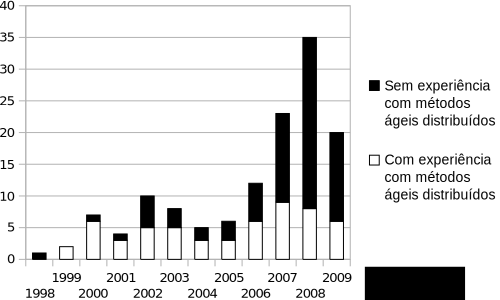
\includegraphics[scale=.65]{agile-distributed}
    \caption{Ano da 1$^{\textrm{a}}$ experiência com métodos ágeis com
      experiência distribuída ou não}
    \label{fig:agile-firstxp}
  \end{minipage}
  \begin{minipage}[t]{0.4\linewidth}
    \centering
    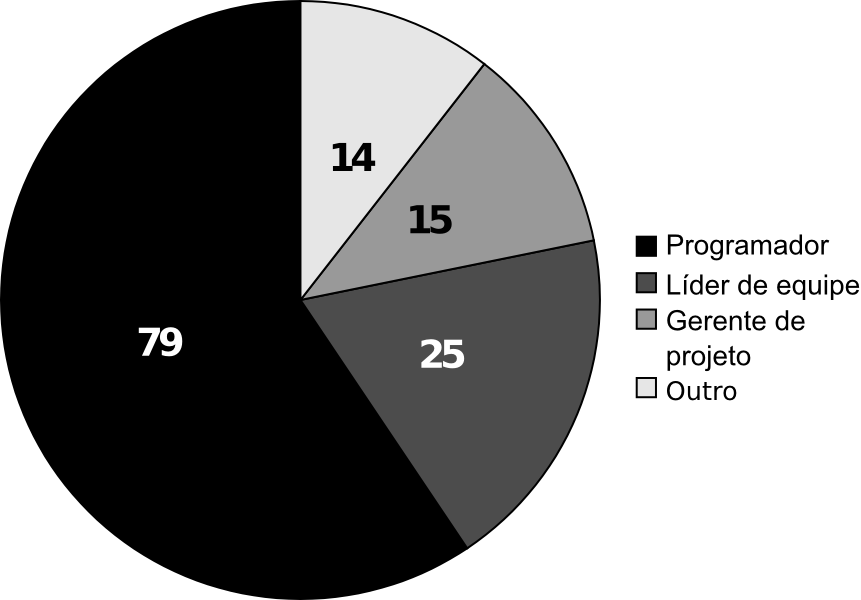
\includegraphics[scale=.60]{agile-roles}
    \caption{Distribuição dos papéis discriminados pela comunidade de
      métodos ágeis}
    \label{fig:agile-roles}
  \end{minipage}
\end{figure}

A maioria dos participantes com alguma experiência teve um contato
muito recente com projetos ágeis. A Figura~\ref{fig:agile-firstxp}
mostra que a primeira experiência da maioria dos participantes com
métodos ágeis só se deu após 2006. Também pode-se notar que há uma
regularidade na quantidade de pessoas com experiência em métodos ágeis
distribuídos independente de seu primeiro ano de experiência com
métodos ágeis. Isso sugere que não houve um aumento sensível no uso de
projetos ágeis distribuídos.

% TODO Regularidade questionável. Deixar mais claro

A Figura~\ref{fig:agile-roles} apresenta a proporção de papéis que os
participantes cumprem em seus projetos ágeis. A maioria se classifica
como programadores. Esse resultado contrasta com a variedade de papéis
acumulados na pesquisa direcionada à comunidade de software
livre. Essa diferença parece ser consequência da prática ``Time
completo'' defendida por Kent Beck~\cite{XP01}. De acordo com essa
prática, uma boa equipe de XP não tem papéis fixos mas deve se adaptar
para extrair o melhor de cada membro da equipe de forma que qualquer
um possa realizar qualquer tarefa caso eles sejam os mais indicados
para isso. Com essa prática, membros de uma equipe de métodos ágeis
são apenas desenvolvedores que contribuem para o projeto. Isso pode
justificar o número reduzido de papéis descritos.

% XXX Fazer uma figura para distribuição dos tamanhos de equipes

Quando se fala de tamanhos de equipe, grupos menores são os mais
comuns. 37\% dos participantes disseram trabalhar com equipes entre 1
e 5 pessoas. 46\% anunciou participar de equipes entre 6 e 10 pessoas,
13\% em equipes de até 20 pessoas e apenas 4\% eram partes de equipes
de mais de 20 pessoas. Isso mostra que equipes de métodos ágeis ainda
são, em grande maioria, equipes pequenas como descritas originalmente.

Aproximadamente 70\% dessas equipes têm comunicação face a face com
seus clientes e consideram que esse canal de comunicação é 67\%
eficaz. Correios eletrônicos, ferramentas de rastreamento de problemas
e telefones acumulam mais 19\% da comunicação entre a equipe e seus
clientes com apenas 54\%, 50\% e 35\% de eficácia respectivamente. O
resto dos canais foram omitidos já que não forneceram dados
relevantes.

Em ambientes distribuídos, os resultados mostram que não há nenhum
consenso com relação à melhor ferramenta de comunicação na equipe. Não
há nenhum canal claramente preferido nem considerado mais eficaz. No
entanto, existe um que é claramente menos eficaz. Para comunicação
entre os membros de uma equipe distribuída, correios eletrônicos
compartilham uma parte razoável das experiências (19\%) mas são
considerados em torno de 31\% eficazes, que é um valor bem menor do
que a maioria dos outros canais.

A ineficácia desse canal de comunicação pode ajudar a explicar porque
56\% dos participantes declararam que ``descobrir o que o
usuário/cliente precisa/quer'' é o maior problema em projetos ágeis. O
segundo e terceiro maior problema são ``estar sincronizado com outros
colaboradores para atingir um objetivo em comum'' e ``descobrir qual é
a próxima tarefa a ser feita'' respectivamente.

Com relação às ferramentas úteis para ajudar praticantes de métodos
ágeis, os resultados foram muito similares aos resultados coletados na
pesquisa para software livre. As ferramentas mais úteis para
praticantes de métodos ágeis são exatamente as mesmas do que para
contribuidores de software livre. Mensagem ou correio eletrônico em
caso de falhas na construção do projeto lidera o ranking seguidos de
estado do projeto dinâmico e gestão do controle de problemas pelas
mensagens de mudanças.

Não é nenhuma surpresa que, para os 35\% dos praticantes de métodos
ágeis que contribuem com projetos livres, os problemas encontrados em
seus ambientes livres são os mesmo do que em seus ambientes ágeis. As
ferramentas para reduzir seus problemas em projetos livres também são
exatamente iguais. No entanto, tal semelhança não se deve ao fato de
participantes considerarem seus projetos livres como ágeis. Em média,
os participantes consideram que seus projetos livres são apenas 56\%
ágeis. Esse nível de não agilidade pode indicar que métodos ágeis e
projetos livres tem problemas em comum que ainda não foram resolvidos.

\section{Conclusão da análise}
\label{sec:proposta}

De posse dos resultados apresentados, fica fácil perceber que a
mentalidade das duas comunidades é semelhante já que ambas
compartilham a mesma visão com respeito aos problemas e às ferramentas
que podem ajudar a contornar esses problemas. No entanto, do ponto de
vista dos princípios e das práticas nas quais cada comunidade se
apóia, parece que há uma distância considerável. Esses resultados
podem ser indícios de que há uma origem comum entre ambos movimentos
mas propostas distintas que evoluíram por caminhos diferentes.

Como a pesquisa indica, ambas comunidades concordam com relação à
preferência por canais de comunicação onde há um rápido
\textit{feedback}. Esses canais estão mais próximos de uma conversa
com perguntas e respostas rápidas. No entanto, a comunidade de
software livre dá preferência a ferramentas que favorecem a distância
física entre os participantes enquanto praticantes de métodos ágeis
preferem comunicação presencial. Isso pode ser dado à natureza
distribuída dos projetos de software livre em contraste com a adoção
de métodos ágeis em meios empresariais.

Sendo assim, uma forma de aproximar as duas comunidades seria de
tentar apresentar um processo munido de ferramentas que permitam
aplicar os princípios de métodos ágeis em ambientes distribuídos com
contribuições voluntárias. O capítulo a seguir
(Capítulo~\ref{cap:diferencas}) apresenta as diferenças entre métodos
ágeis e software livre. São essas diferenças que esse trabalho se
propôs a explorar.

